% Section VI of draft v5, rewritten (CLAUDE.md §8 item 184). Measured numbers: uav-l2/docs/data/results/baselines.csv
% (ns-3, 2026-10-26). Red [EST]: LM-Tour, estimated by estimate.py, not run. Replace after the run.
\section{Evaluation}
\emph{Setup.} ns-3.46 with \texttt{lr-wpan} (CSMA/CA, ACK, retransmission); channel and radio as in Section~III-B
($\alpha = 3$). Three maps with $K$ = 8, 12 and 16 target clusters (8, 12 and 15 clusters; 45, 66 and 92 critical
cells; capacitated $k$-medoids, at most 80 cells each). Four A2G regimes: $L_{\mathrm{obs}}$ = 0, 9.0, 19.8 and
25.7~dB in (1), calibrated on the ns-3 pass so that the lateral reach $\sqrt{r^2-h^2}$ is 1015, 498, 199 and 99~m,
i.e.\ $r \approx 1000$, 500, 200 and 150~m. Team~1 flies a speed profile (45$^\circ$ bank, $\pm2$\,m/s$^2$), slowing
down to 25~m/s or looping where a cluster would otherwise not be offered one copy of the query (Eq.~(3)); the clue set
is fountain-coded and systematic. One ns-3 run per cluster; 100 paired draws of the matching layer per map; every
scheme sees the same pass bitmaps, coded receptions and draws. Results are exploratory ($N < 120$).

\emph{Schemes.} \emph{LM-Tour + River-FC} (proposed, Section~V, $\xi$ from (5)); \emph{CHORD + River-FC}: the longest
flyable chord through each cluster head, bearings and order chosen jointly to minimise the mean time critical cells
are left behind, River with fountain coding; \emph{FC + gather}: team~1 flies a TSP over the critical cells
themselves and circles each one until its nodes hold enough coded packets, in-cell gathering only;
\emph{FC + DTSP-N}: as FC + gather, but nearby critical cells grouped and served from orbits chosen by a sampled
Dubins TSP with neighbourhoods; \emph{Single pass, no cooperation}: CHORD's flight, each critical cell uses only what
it decoded itself; \emph{No broadcast (rotary TSP)}: team~2 alone visits every critical cell with the full
reference; \emph{Oracle}: team~2 flies straight to the target cell.

\begin{table}[t]\centering\caption{Critical cells complete after the pass (\%) and time from take-off to the last completion (s) versus A2G range, $K = 16$ (92 critical cells). \textcolor{red}{[EST]: estimated.}}\label{tab:complete}
\footnotesize\begin{tabular}{lcccc}\toprule
Scheme & $r=150$ & 200 & 500 & 1000\,m \\\midrule
No cooperation & 0\,\% / -- & 1\,\% / -- & 66\,\% / -- & 100\,\% / -- \\
FC + gather & 100\,\% / 7257 & 100\,\% / 6591 & 100\,\% / 2784 & 100\,\% / 1132 \\
FC + DTSP-N & 100\,\% / 6761 & 100\,\% / 5523 & 100\,\% / 2529 & 100\,\% / 1041 \\
River-FC (CHORD) & 100\,\% / 1395 & 100\,\% / 1398 & 100\,\% / 1204 & 100\,\% / 1052 \\
\textcolor{red}{River-FC + LM-Tour} & \textcolor{red}{100\,\% / 1283} & \textcolor{red}{100\,\% / 1268} & \textcolor{red}{100\,\% / 1082} & \textcolor{red}{100\,\% / 1018} \\
\bottomrule\end{tabular}\end{table}


\subsection{Robustness to the A2G regime}
Table~\ref{tab:complete}: without cooperation every critical cell completes at $r = 1$~km, 66\,\% at 500~m and
almost none at $r \le 200$~m. FC-based schemes complete every critical cell only by circling: the last one completes
2.1--5.2$\times$ later than with River-FC as $r$ shrinks, whereas River-FC's completion grows by only 150--350~s,
because River sources data from the cells under the path, which hear their own segment at any $r$.

\begin{table*}[t]\centering\color{blue}\caption{Mean mission time $T^\star$ (s), 100 paired draws, $K$ = 8 / 12 / 16 clusters. \textcolor{red}{[EST]: estimated, not run.}}\label{tab:tstar}
\setlength{\tabcolsep}{3pt}\footnotesize
\begin{tabular}{lcccc}\toprule
Scheme & $r=1000$ m & 500 & 200 & 150 \\\midrule
\textcolor{red}{LM-Tour + River-FC} & 647 / 686 / 863 & 775 / 942 / 1097 & 822 / 936 / 1143 & 810 / 942 / 1157 \\
{CHORD + River-FC} & 647 / 686 / 863 & 784 / 950 / 1107 & 876 / 975 / 1192 & 872 / 990 / 1215 \\
{FC + gather} & 660 / 815 / 949 & 1138 / 1451 / 1801 & 2285 / 3288 / 3964 & 2463 / 3460 / 4368 \\
{FC + DTSP-N} & 708 / 805 / 967 & 1078 / 1388 / 1750 & 1904 / 2482 / 3469 & 2190 / 3248 / 4468 \\
{Single pass, no cooperation} & 650 / 687 / 862 & 1379 / 2030 / 2549 & 3711 / 5277 / 6298 & 3860 / 5308 / 6358 \\
{No broadcast (rotary TSP)} & 2926 / 4168 / 5169 & 2926 / 4168 / 5169 & 2926 / 4168 / 5169 & 2926 / 4168 / 5169 \\
{Oracle} & 322 / 402 / 404 & 322 / 402 / 404 & 322 / 402 / 404 & 322 / 402 / 404 \\
\bottomrule\end{tabular}\end{table*}


\begin{figure}[t]\centering
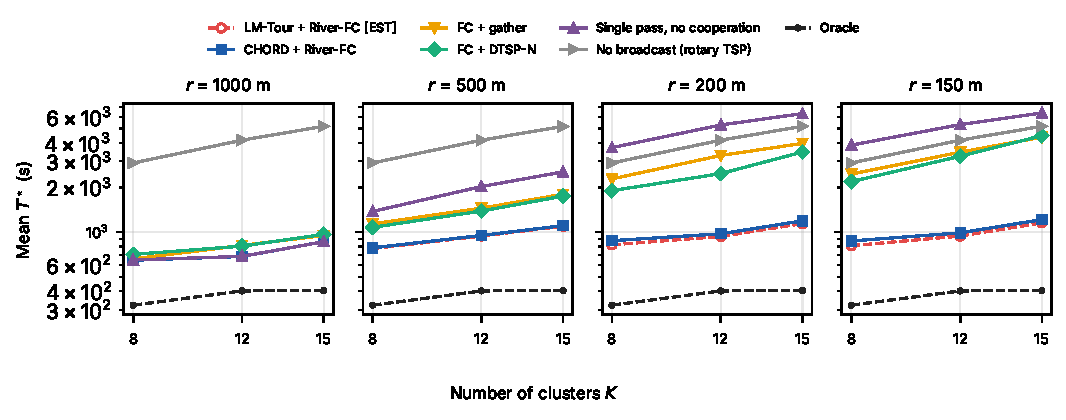
\includegraphics[width=\columnwidth]{figs/fig6-tstar-vs-k-4ranges.pdf}
\caption{Mean $T^\star$ versus the number of clusters, per A2G range (log scale). LM-Tour: estimated
\textcolor{red}{[EST]}. Oracle knows the target cell.}\label{fig:mission}
\end{figure}

\subsection{Mission level}
Table~\ref{tab:tstar}, Fig.~\ref{fig:mission}: the single-pass architecture with River-FC is 3.3--6.0$\times$ faster
than having no broadcast phase. Against the FC baselines it is 2--15\,\% faster at $r = 1$~km and 27--72\,\% faster
at $r \le 500$~m, and the gap widens with $K$: CHORD's flight stays 782 / 1152 / 1415~s at every $r$, while FC's grows
2--6$\times$. Without cooperation the same flight is 1.8--5.4$\times$ slower at $r \le 500$~m.
\textcolor{red}{[EST] LM-Tour shortens $T^\star$ by a further 1--7\,\% at $r \le 500$~m (no change at 1~km), by
bringing the path within direct hearing of each landmark. Estimated, to be measured.}
